


\begin{frame}{Table of Contents}
   \begin{block}{What about threads in PETSc?} \end{block}
   \begin{block}{What about all those branches in the repository?} \end{block}
   \begin{block}{What kind of questions do users have?} \end{block}
   \begin{block}{What is Firetran?} \end{block}
\end{frame}


%
% Threads
%
\section{PETSc and Threads}

\begin{frame}{PETSc Tutorial}
   \begin{center} \Large \textbf{What about threads in PETSc?} \end{center}

\end{frame}


\begin{frame}[fragile]{PETSc and Threads}

 \begin{block}{Competing Threading Approaches}
  \begin{itemize}
   \item pthread
   \item OpenMP
   \item C++11 threads
   \item Compiler magic
  \end{itemize}
 \end{block}

 %\pause
 \begin{block}{Issues with Threads}
  \begin{itemize}
   \item Problematic across compilers
   \item Data locality
   \item Thread ownership
   \item Software interface
  \end{itemize}
 \end{block}

 %\pause
  \begin{block}{Assumption for Subsequent Discussion}
  \begin{itemize}
   \item Primary Goal: Get the science done!
   \item 10 percent performance difference is \textbf{not significant}
  \end{itemize}
 \end{block}

\end{frame}


\begin{frame}[fragile]{PETSc and Threads}
  \begin{block}{When to Use Threads After All?}
    \begin{itemize}
     \item Distributed Memory: Need MPI anyway
     %\pause
     \item Shared Memory: MPI for multi-socket systems for NUMA reasons
     %\pause
     \item 1-Socket Machines: If a 2-5x gain is critical, use a cluster!
    \end{itemize}
  \end{block}

  \begin{center}
    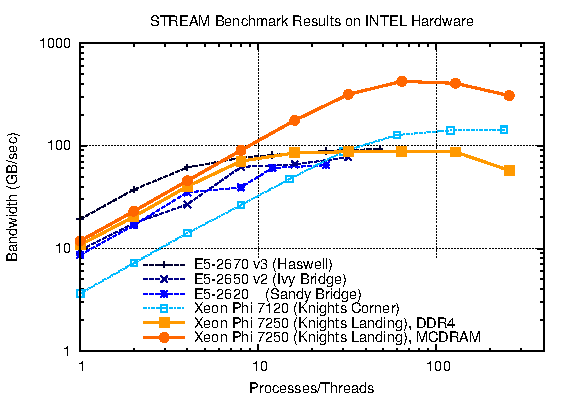
\includegraphics[width=0.55\textwidth]{figures/stream}
  \end{center}
  
\end{frame}


\begin{frame}[fragile]{Threads and Library Interfaces}

 \begin{block}{Attempt 1}
  \begin{itemize}
   \item Library spawns threads
  \end{itemize}
 \end{block}

   \begin{lstlisting}
  void library_func(double *x, int N) {
    #pragma omp parallel for
    for (int i=0; i<N; ++i) x[i] = something_complicated();
  }
  \end{lstlisting}

  %\pause
  
  \begin{block}{Problems}
   \begin{itemize}
    \item Call from multi-threaded environment?
   \begin{lstlisting}
  void user_func(double **y, int N) {
    #pragma omp parallel for
    for (int j=0; j<M; ++j) library_func(y[j], N);
  }
  \end{lstlisting}
    \item Incompatible OpenMP runtimes (e.g. GCC vs. ICC)
   \end{itemize}
 \end{block}

\end{frame}

\begin{frame}[fragile]{Threads and Library Interfaces}

 \begin{block}{Attempt 2}
  \begin{itemize}
   \item Use pthreads/TBB/etc. instead of OpenMP to spawn threads
   \item Fixes incompatible OpenMP implementations (probably)
  \end{itemize}
 \end{block}

  %\pause
  \begin{block}{Problems}
   \begin{itemize}
    \item Still a problem with multi-threaded user environments
   \begin{lstlisting}
  void user_func(double **y, int N) {
    #pragma omp parallel for
    for (int j=0; j<M; ++j) library_func(y[j], N);
  }
   \end{lstlisting}
  \end{itemize}
 \end{block}

\end{frame}


\begin{frame}[fragile]{Threads and Library Interfaces}

 \begin{block}{Attempt 3}
  \begin{itemize}
   \item Hand back thread management to user
  \end{itemize}
 \end{block}

  \begin{lstlisting}
  void library_func(ThreadInfo ti, double *x, int N) {
    int start = compute_start_index(ti, N);
    int stop  = compute_stop_index(ti, N);
    for (int i=start; i<stop; ++i)
      x[i] = something_complicated();
  }
  \end{lstlisting}

  %\pause
  \begin{block}{Implications}
   \begin{itemize}
    \item Users can use their favorite threading model
    \item API requires one extra parameter
    \item Extra boilerplate code required in user code
  \end{itemize}
 \end{block}
\end{frame}


\begin{frame}[fragile]{Threads and Library Interfaces}

 \begin{block}{Reflection}
  \begin{itemize}
   \item Extra thread communication parameter
    \begin{lstlisting}
void library_func(ThreadInfo ti, double *x, int N) {...}
    \end{lstlisting}
    %\pause
   \item Rename thread management parameter
    \begin{lstlisting}
void library_func(Thread_Comm c, double *x, int N) {...}
    \end{lstlisting}
    %\pause
   \item Compare:
    \begin{lstlisting}
void library_func(MPI_Comm comm, double *x, int N) {...}
    \end{lstlisting}
  \end{itemize}
 \end{block}

 %\pause
  \begin{block}{Conclusion}
   \begin{itemize}
    \item Prefer flat MPI over MPI+OpenMP for a composable software stack
    \item MPI automatically brings better data locality
  \end{itemize}
 \end{block}

\end{frame}




%
% Git branches
%
\section{PETSc and Git}

\begin{frame}{PETSc}
   \begin{center} \Large \textbf{What about all those branches in the repository?} \end{center}
\end{frame}



\begin{frame}{PETSc and Git}
  \begin{block}{PETSc's Workflow}
  \begin{center}
    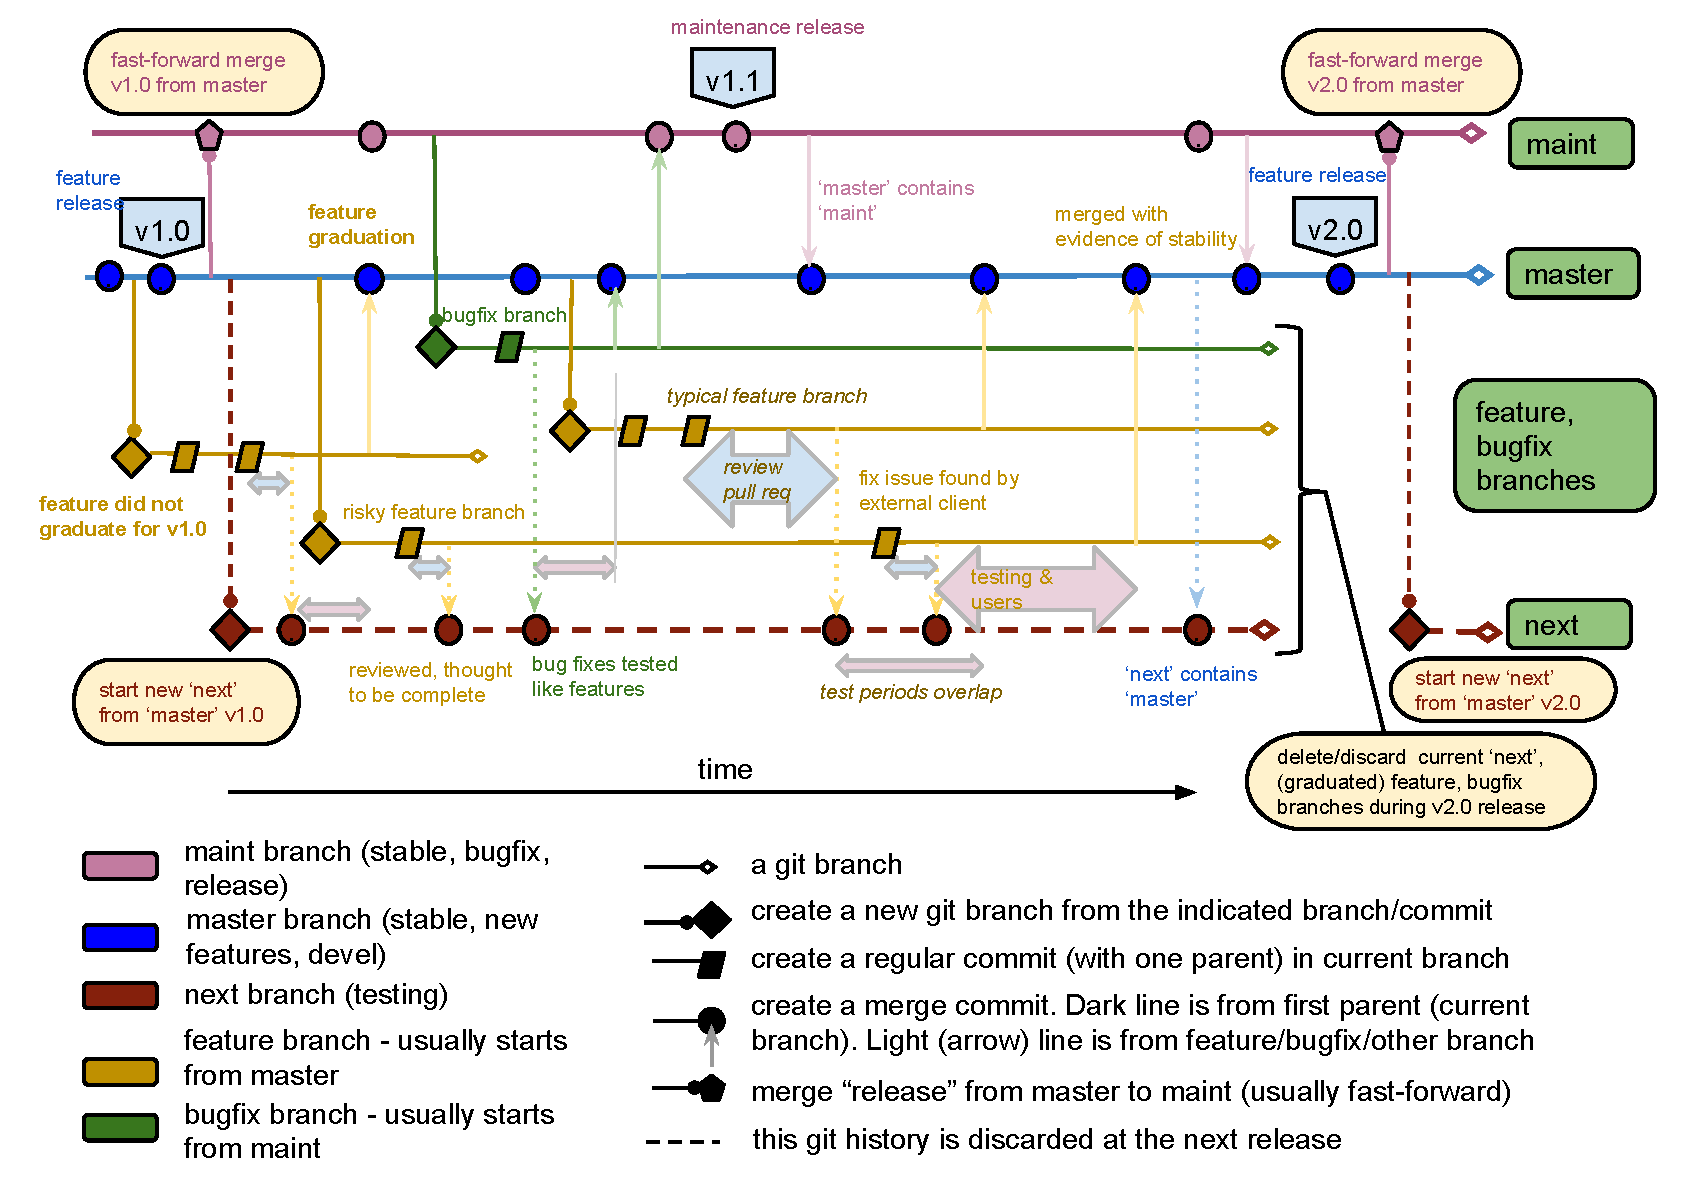
\includegraphics[width=0.85\textwidth]{figures/gitworkflows-satish}
  \end{center}
  \end{block}

  \begin{flushright} \vspace*{-0.5cm}
   \textit{Git is the perl of revision control systems.}
  \end{flushright}
\end{frame}


\begin{frame}{PETSc and Git}
  \begin{center}
    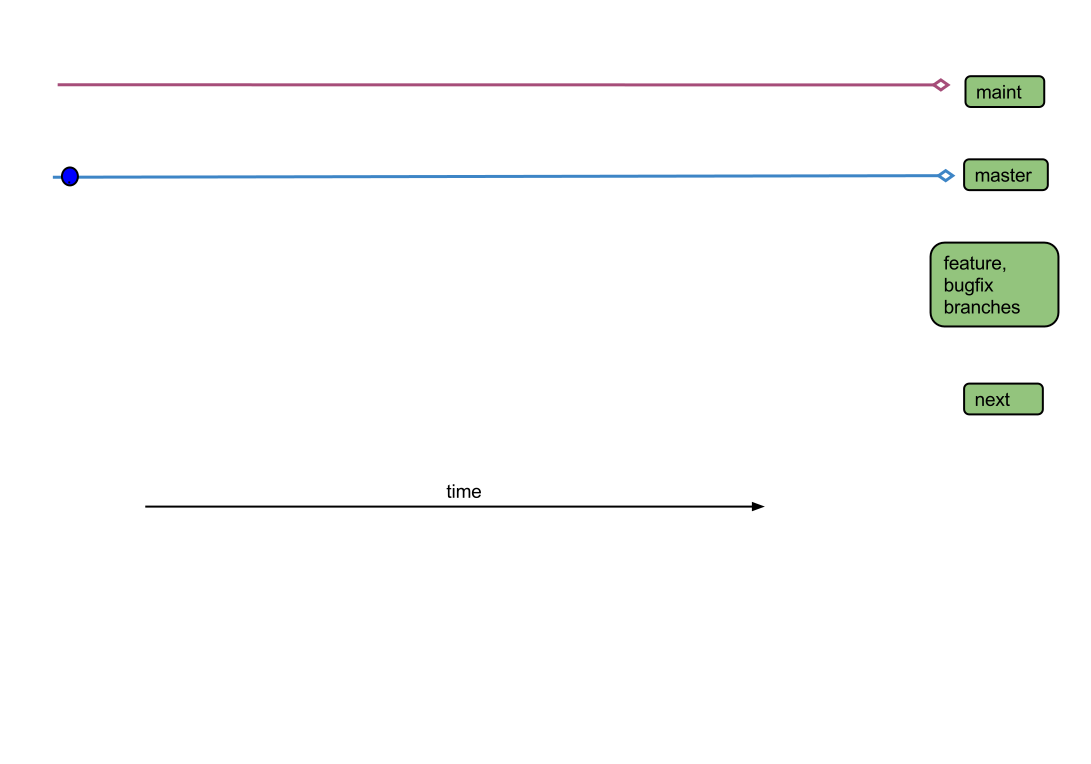
\includegraphics[width=0.99\textwidth]{figures/gitworkflows-45}
  \end{center}
  \begin{flushright} \vspace*{-0.5cm}
   \textit{Oh, yes we all do need that push!}
  \end{flushright}
\end{frame}

\begin{frame}{PETSc and Git}
  \begin{center}
    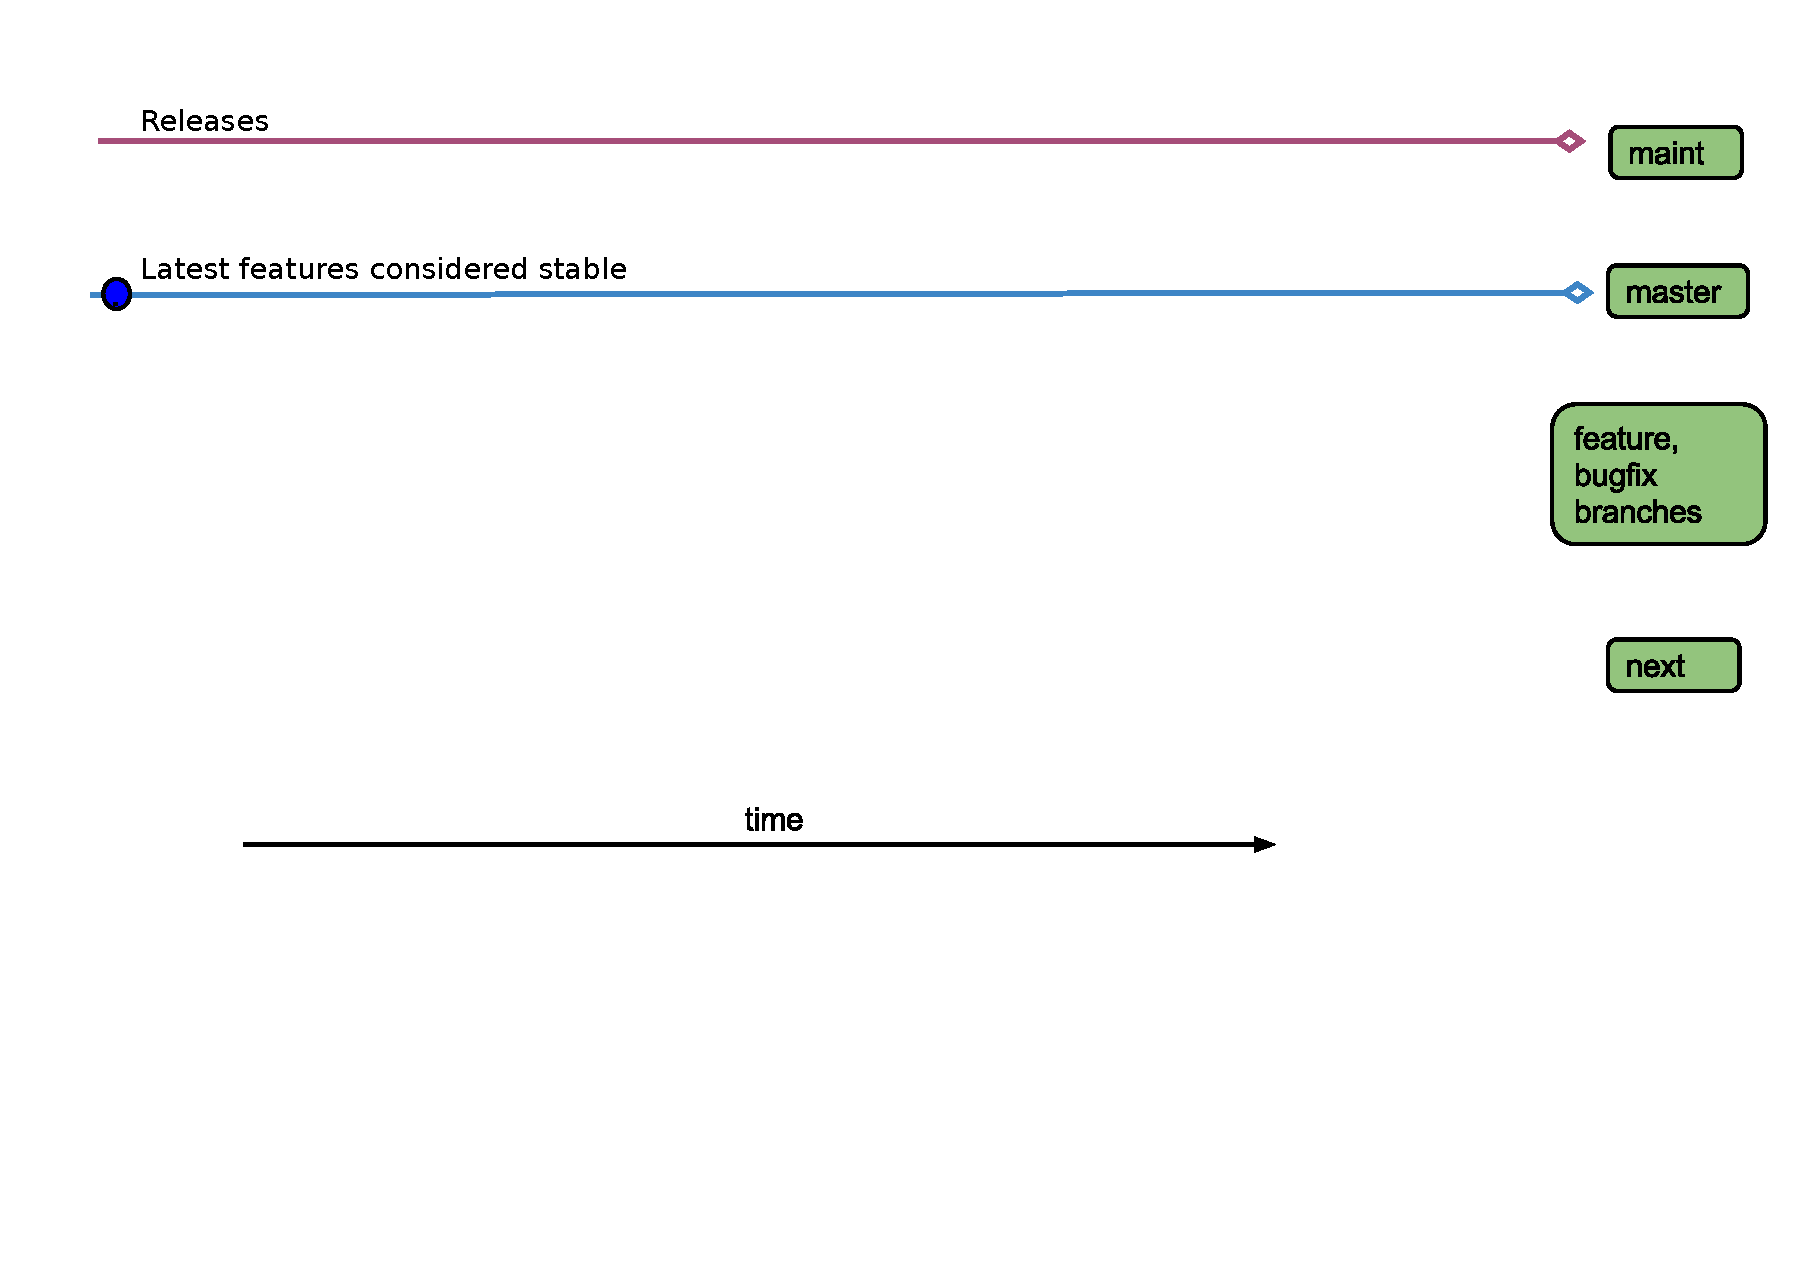
\includegraphics[width=0.99\textwidth]{figures/gitworkflows-50}
  \end{center}
  \begin{flushright} \vspace*{-0.5cm}
   \textit{It's like we only offer the black belt for people who currently have no belts.}
  \end{flushright}
\end{frame}

\begin{frame}{PETSc and Git}
  \begin{center}
    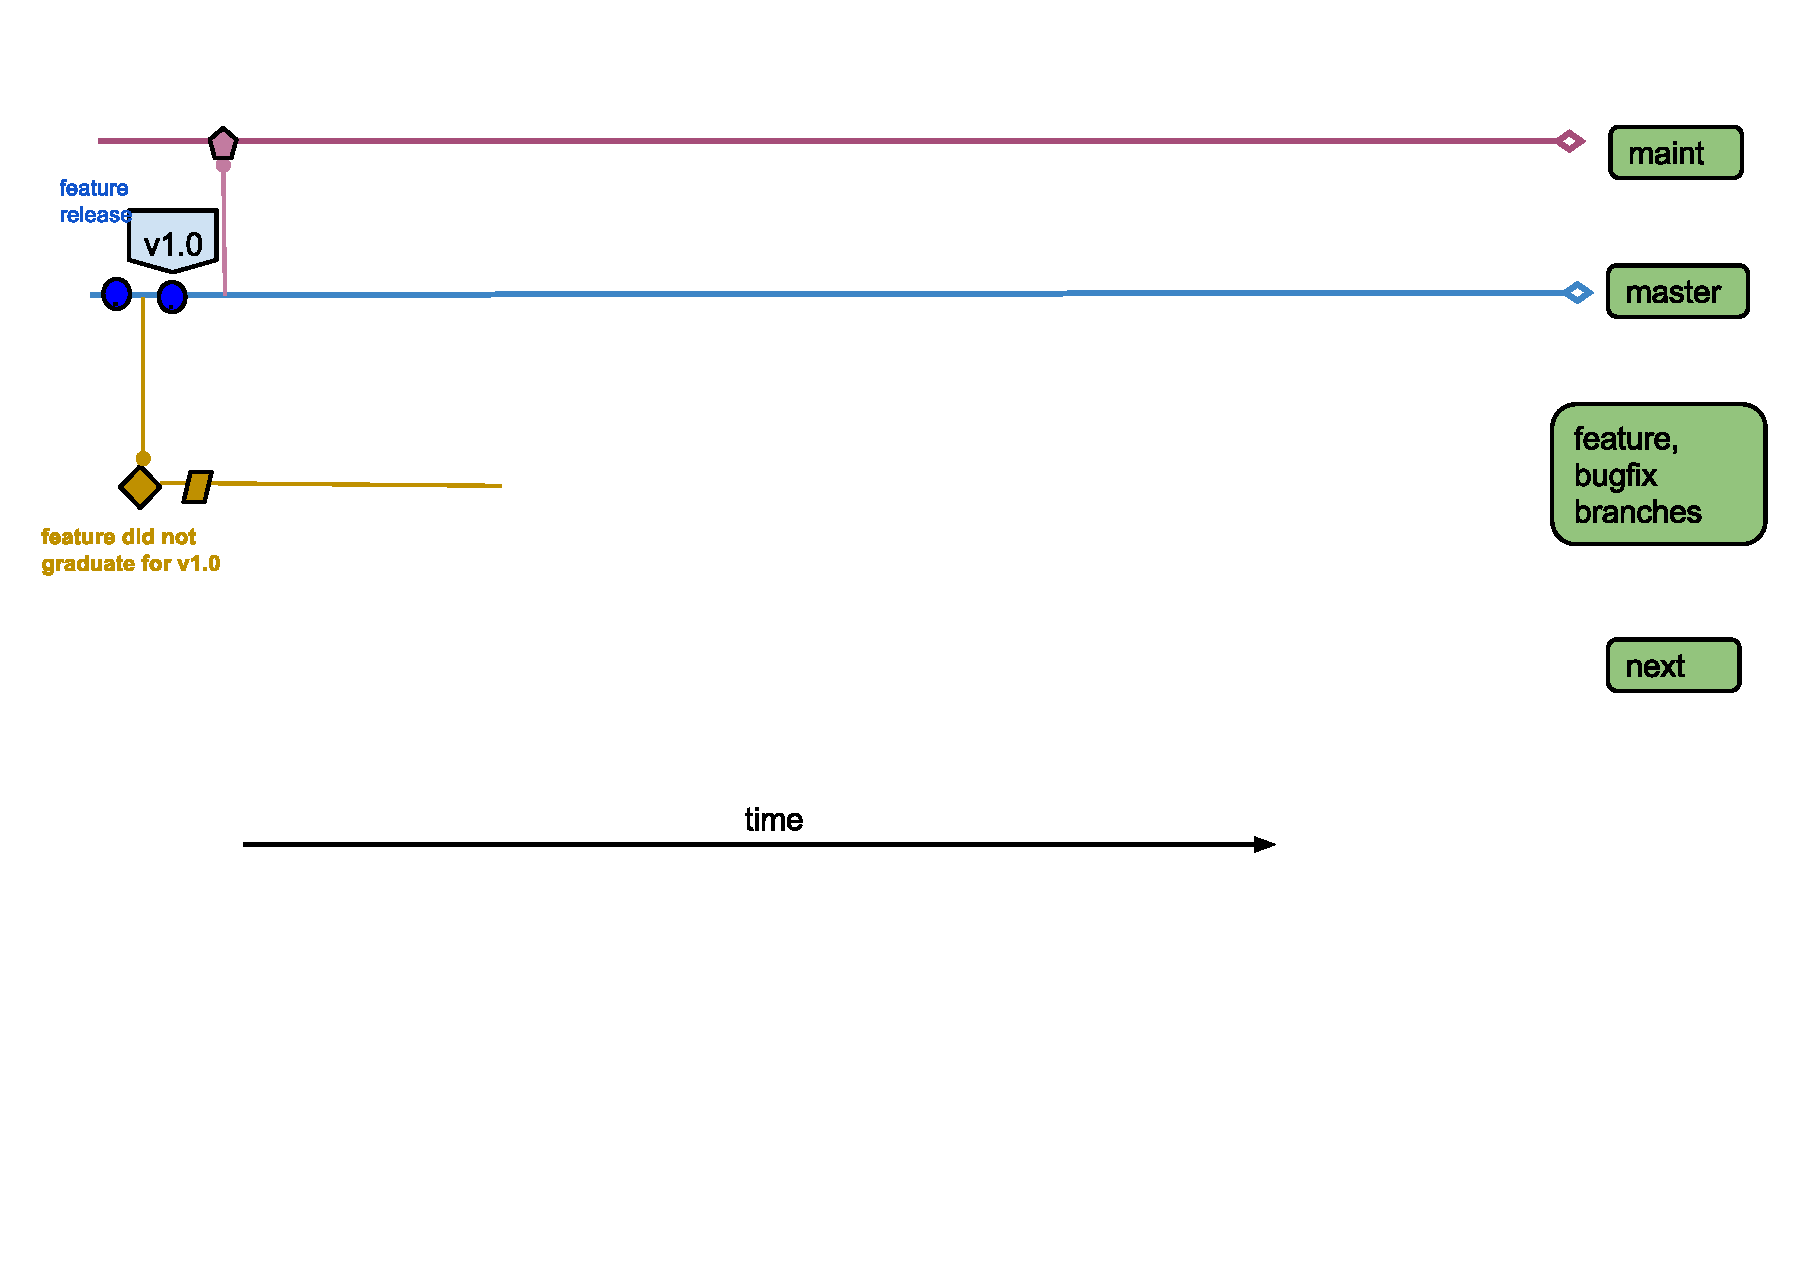
\includegraphics[width=0.99\textwidth]{figures/gitworkflows-55}
  \end{center}
  \begin{flushright} \vspace*{-0.5cm}
   \textit{If it ain't in email or slashdot then I ain't read it :-)}
  \end{flushright}
\end{frame}

\begin{frame}{PETSc and Git}
  \begin{center}
    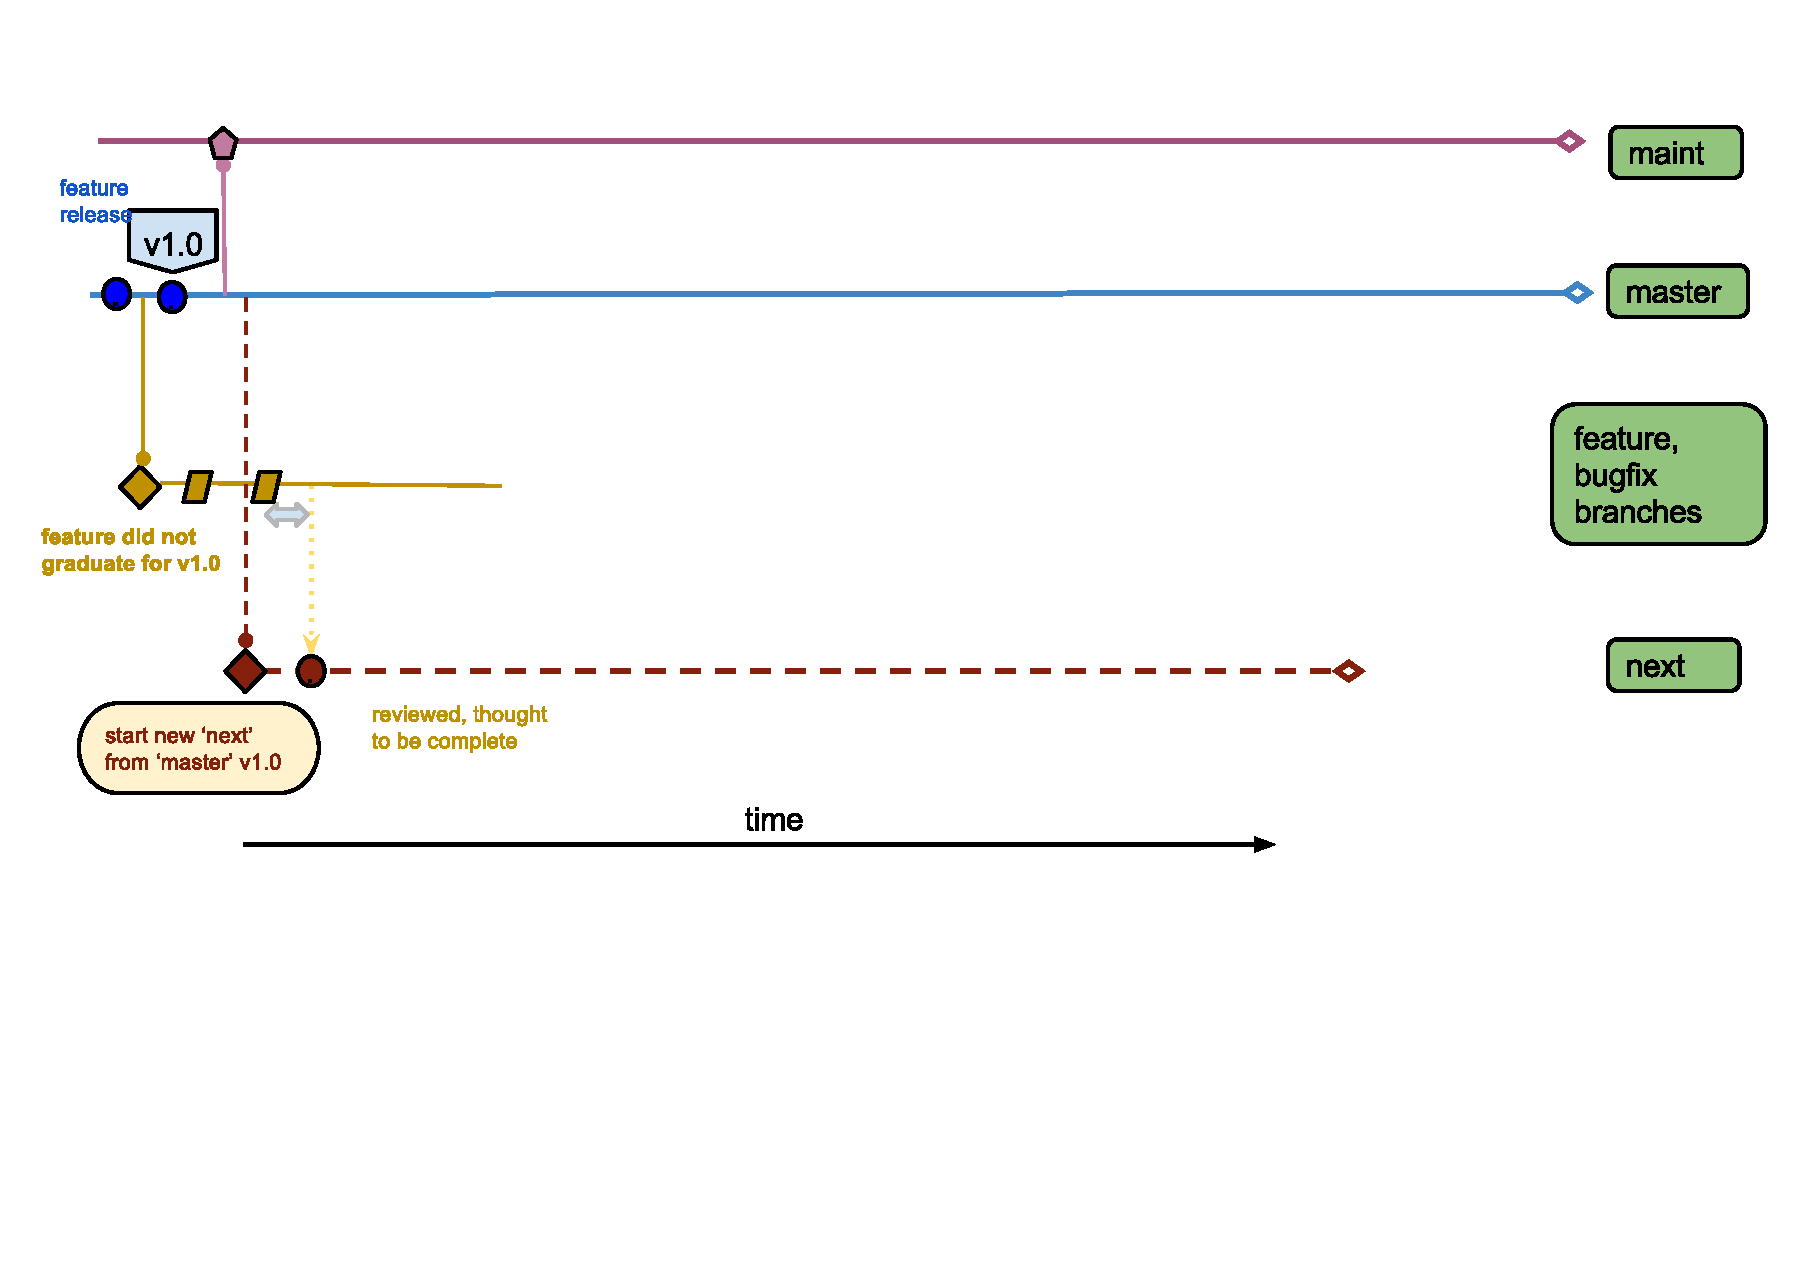
\includegraphics[width=0.99\textwidth]{figures/gitworkflows-58}
  \end{center}
  \begin{flushright} \vspace*{-0.5cm}
   \textit{I have now permanently blackholed all email dealing with cygwin.}
  \end{flushright}
\end{frame}

\begin{frame}{PETSc and Git}
  \begin{center}
    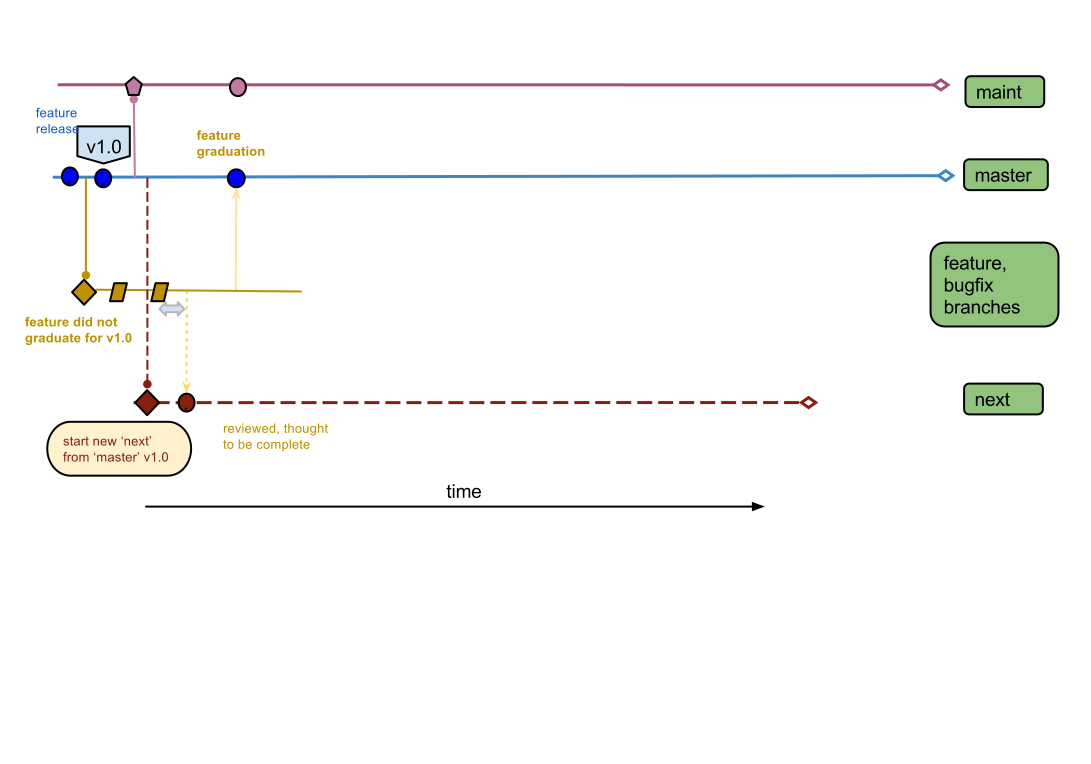
\includegraphics[width=0.99\textwidth]{figures/gitworkflows-60}
  \end{center}
  \begin{flushright} \vspace*{-0.5cm}
   \textit{Peter, Matt gave some bad advice.}
  \end{flushright}
\end{frame}

\begin{frame}{PETSc and Git}
  \begin{center}
    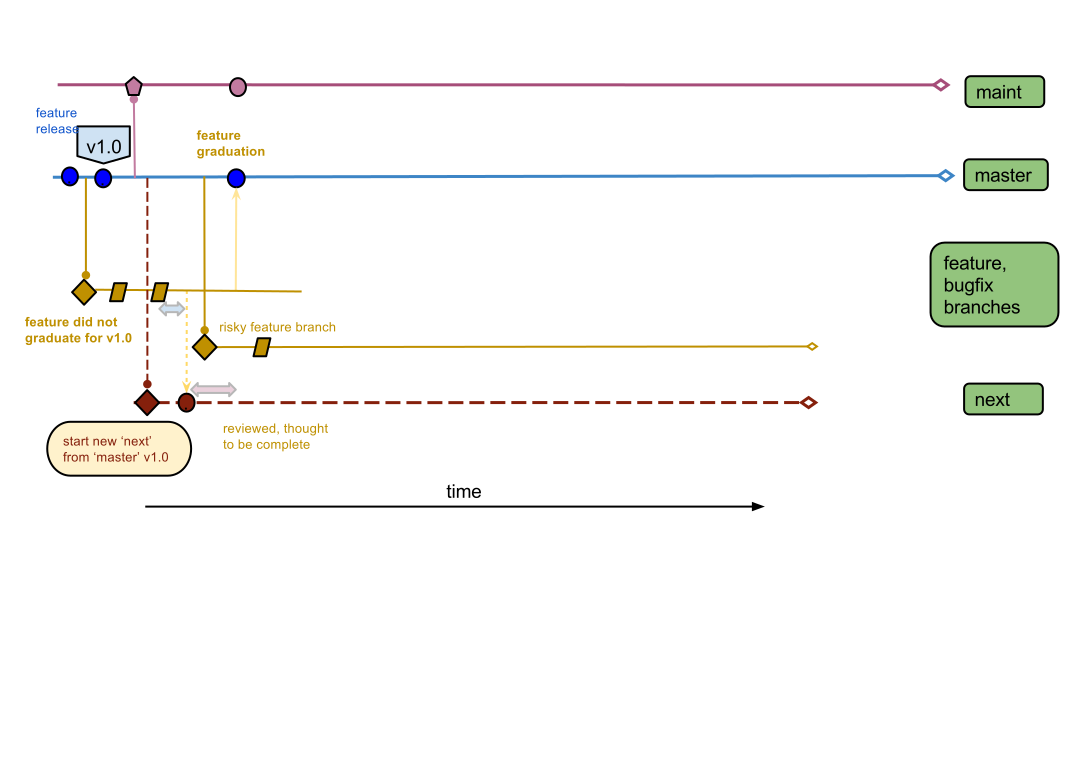
\includegraphics[width=0.99\textwidth]{figures/gitworkflows-65}
  \end{center}
  \begin{flushright} \vspace*{-0.5cm}
   \textit{Satish, please put this in next with the other six million branchs.}
  \end{flushright}
\end{frame}

\begin{frame}{PETSc and Git}
  \begin{center}
    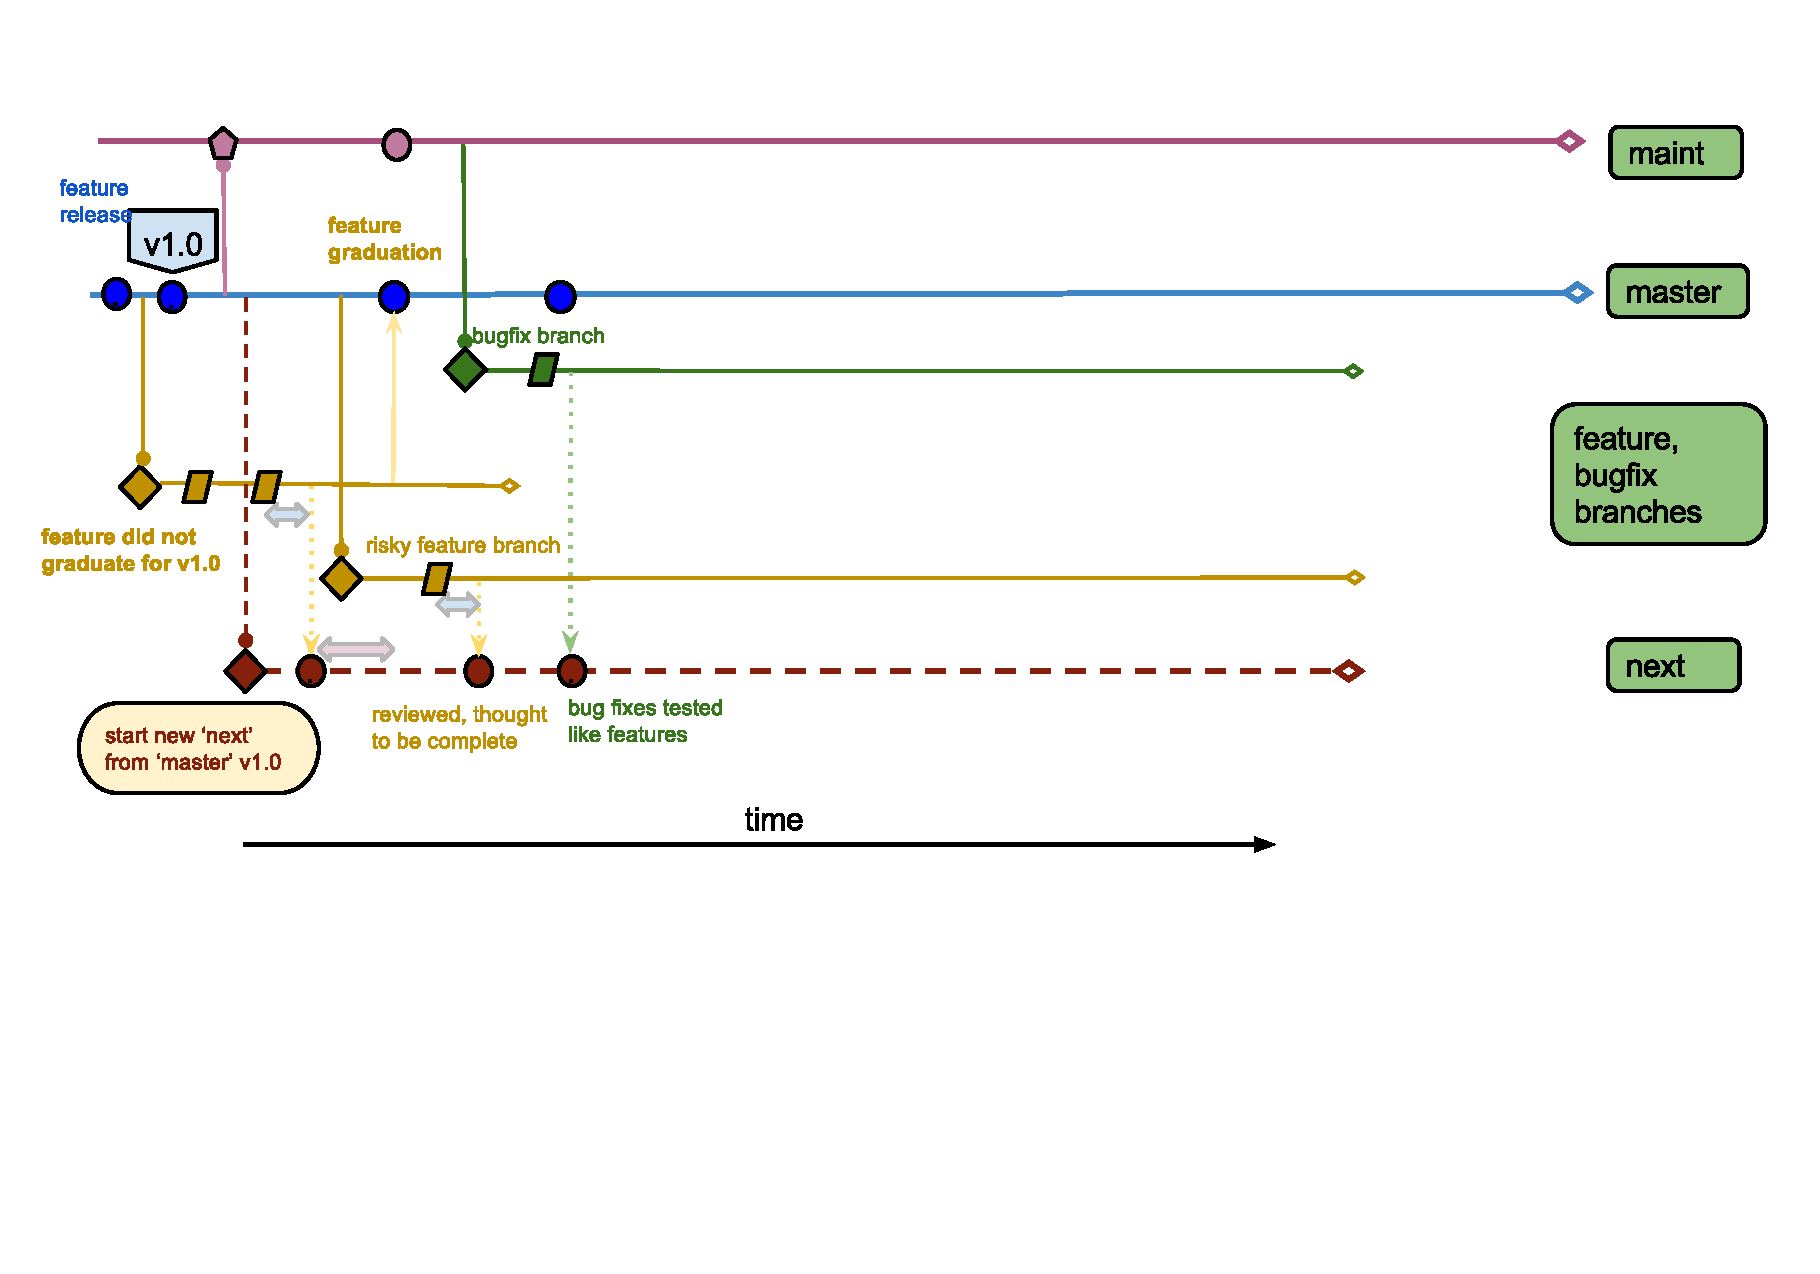
\includegraphics[width=0.99\textwidth]{figures/gitworkflows-70}
  \end{center}
  \begin{flushright} \vspace*{-0.5cm}
   \textit{Don't tell anyone that I put a printf in here}
  \end{flushright}
\end{frame}

\begin{frame}{PETSc and Git}
  \begin{center}
    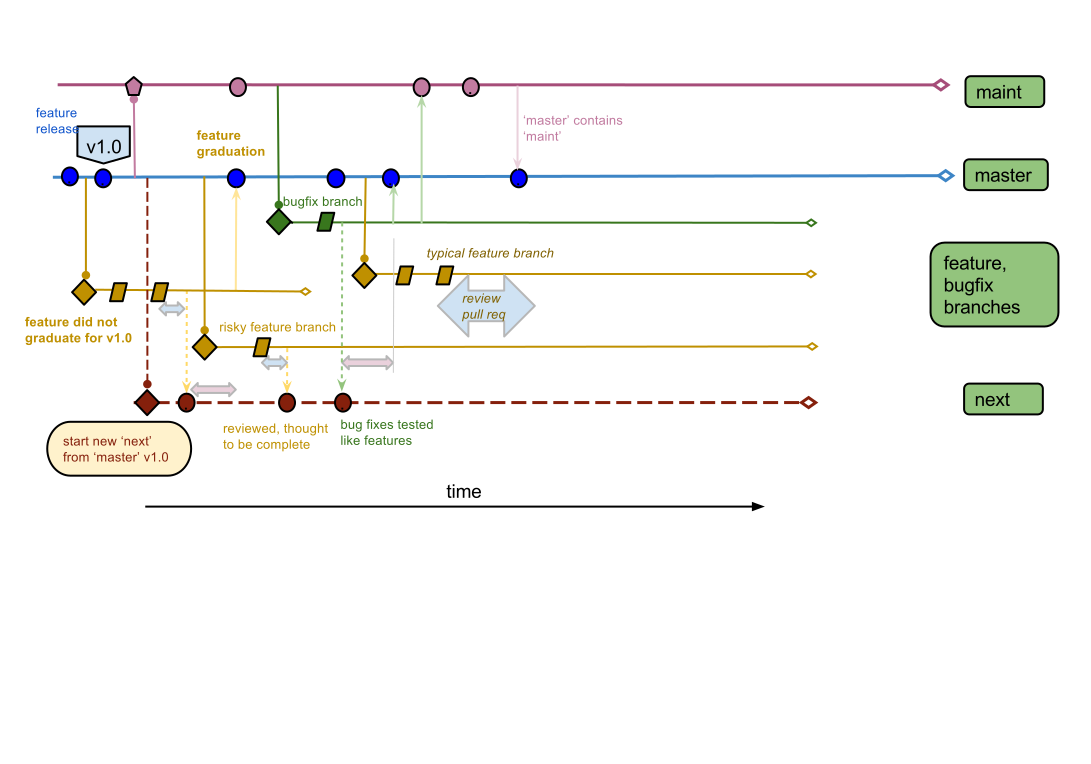
\includegraphics[width=0.99\textwidth]{figures/gitworkflows-75}
  \end{center}
  \begin{flushright} \vspace*{-0.5cm}
   \textit{I won't call the ICNTL() monstrosity in MUMPS an interface :-)}
  \end{flushright}
\end{frame}

\begin{frame}{PETSc and Git}
  \begin{center}
    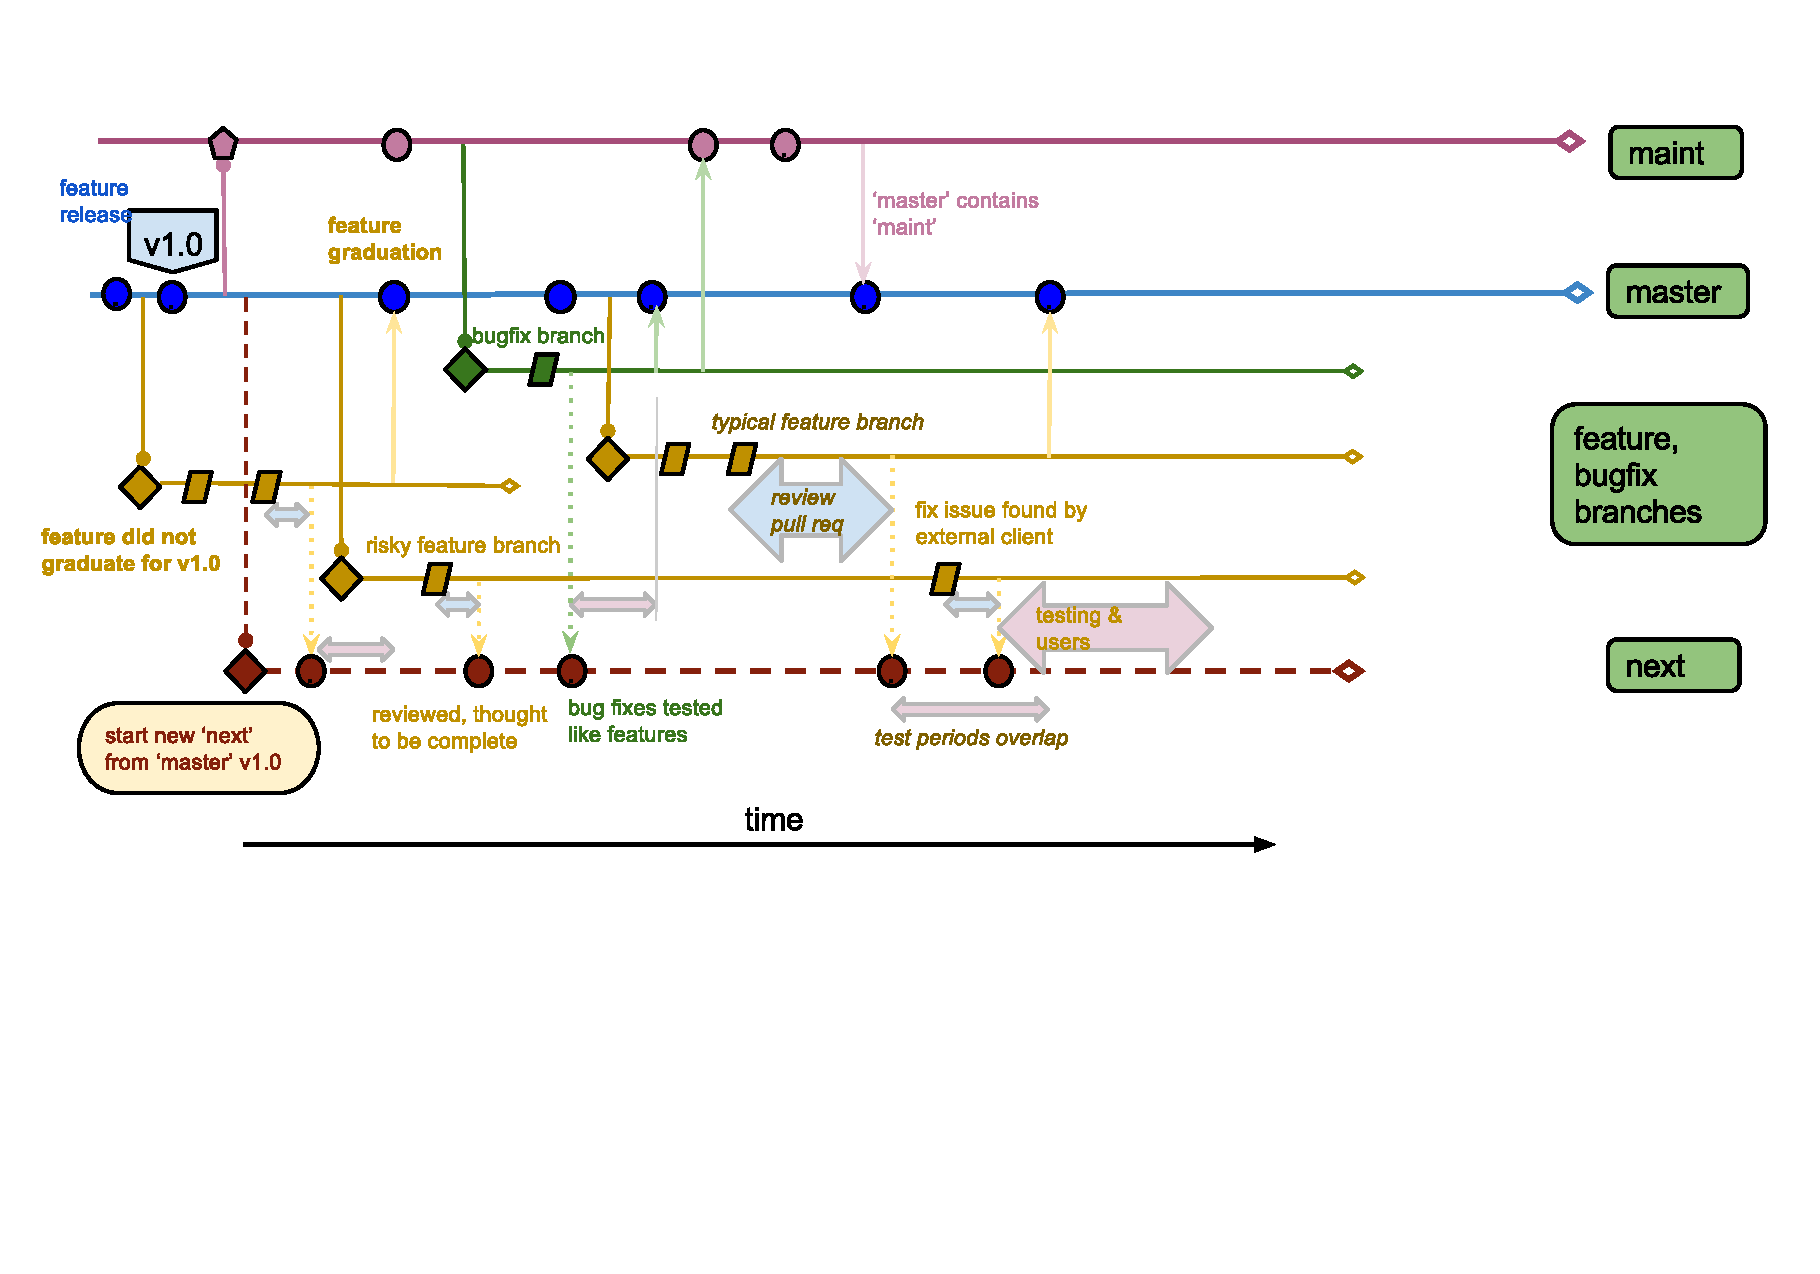
\includegraphics[width=0.99\textwidth]{figures/gitworkflows-80}
  \end{center}
  \begin{flushright} \vspace*{-0.5cm}
   \textit{That is all I know about valgrind and it has saved my bacon many times.}
  \end{flushright}
\end{frame}

\begin{frame}{PETSc and Git}
  \begin{center}
    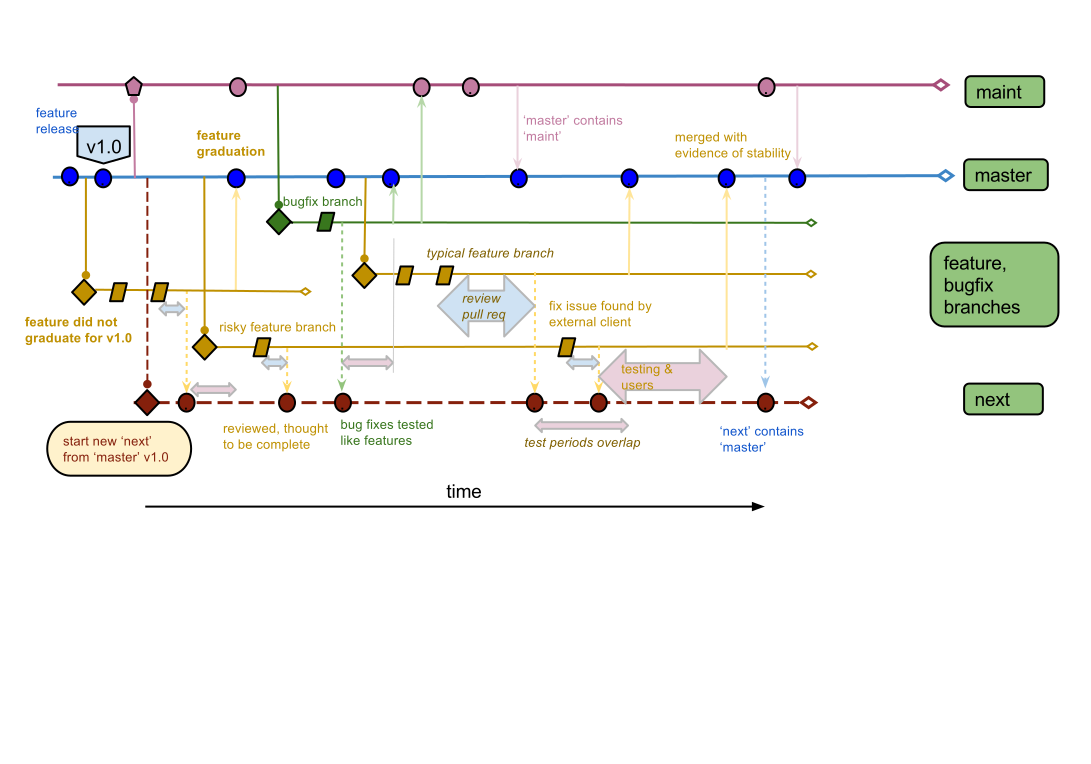
\includegraphics[width=0.99\textwidth]{figures/gitworkflows-85}
  \end{center}
  \begin{flushright} \vspace*{-0.5cm}
   \textit{Stop right here. 99.9\% of the time what you describe should not happen}
  \end{flushright}
\end{frame}

\begin{frame}{PETSc and Git}
  \begin{center}
    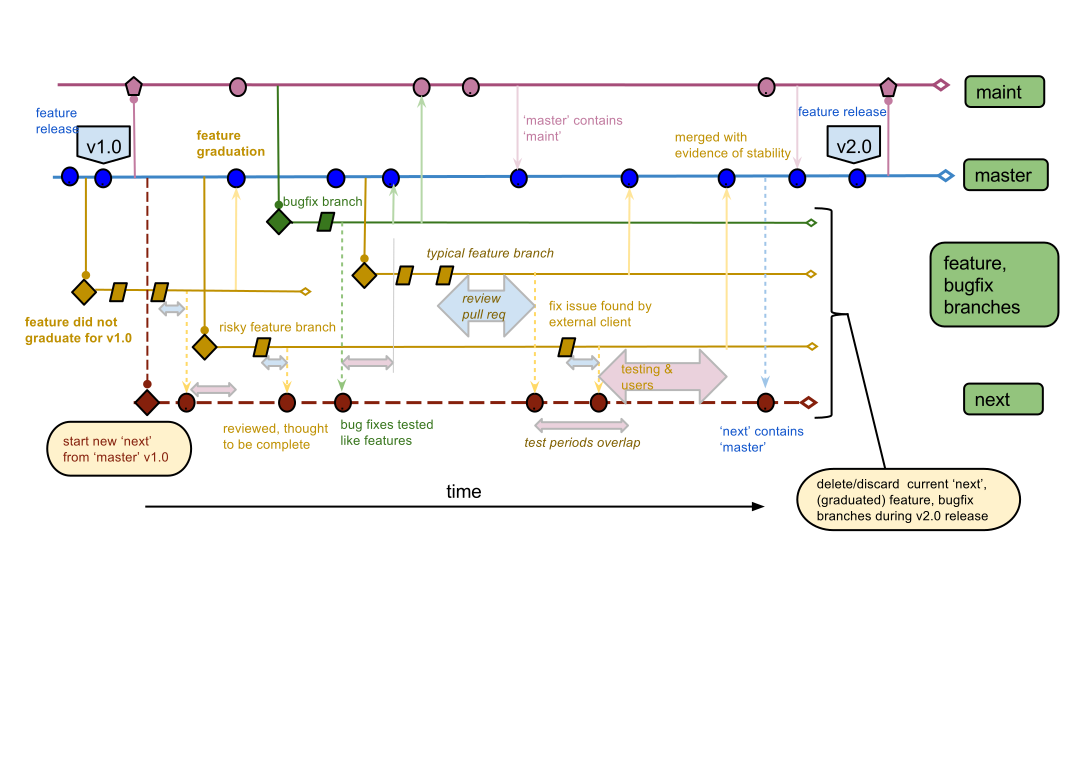
\includegraphics[width=0.99\textwidth]{figures/gitworkflows-90}
  \end{center}
  \begin{flushright} \vspace*{-0.8cm}
   \textit{Git is TeX, what we need is someone to come along\\ and produce LaGit and thus make it usable.}
  \end{flushright}
\end{frame}

\begin{frame}{PETSc and Git}
  \begin{center}
    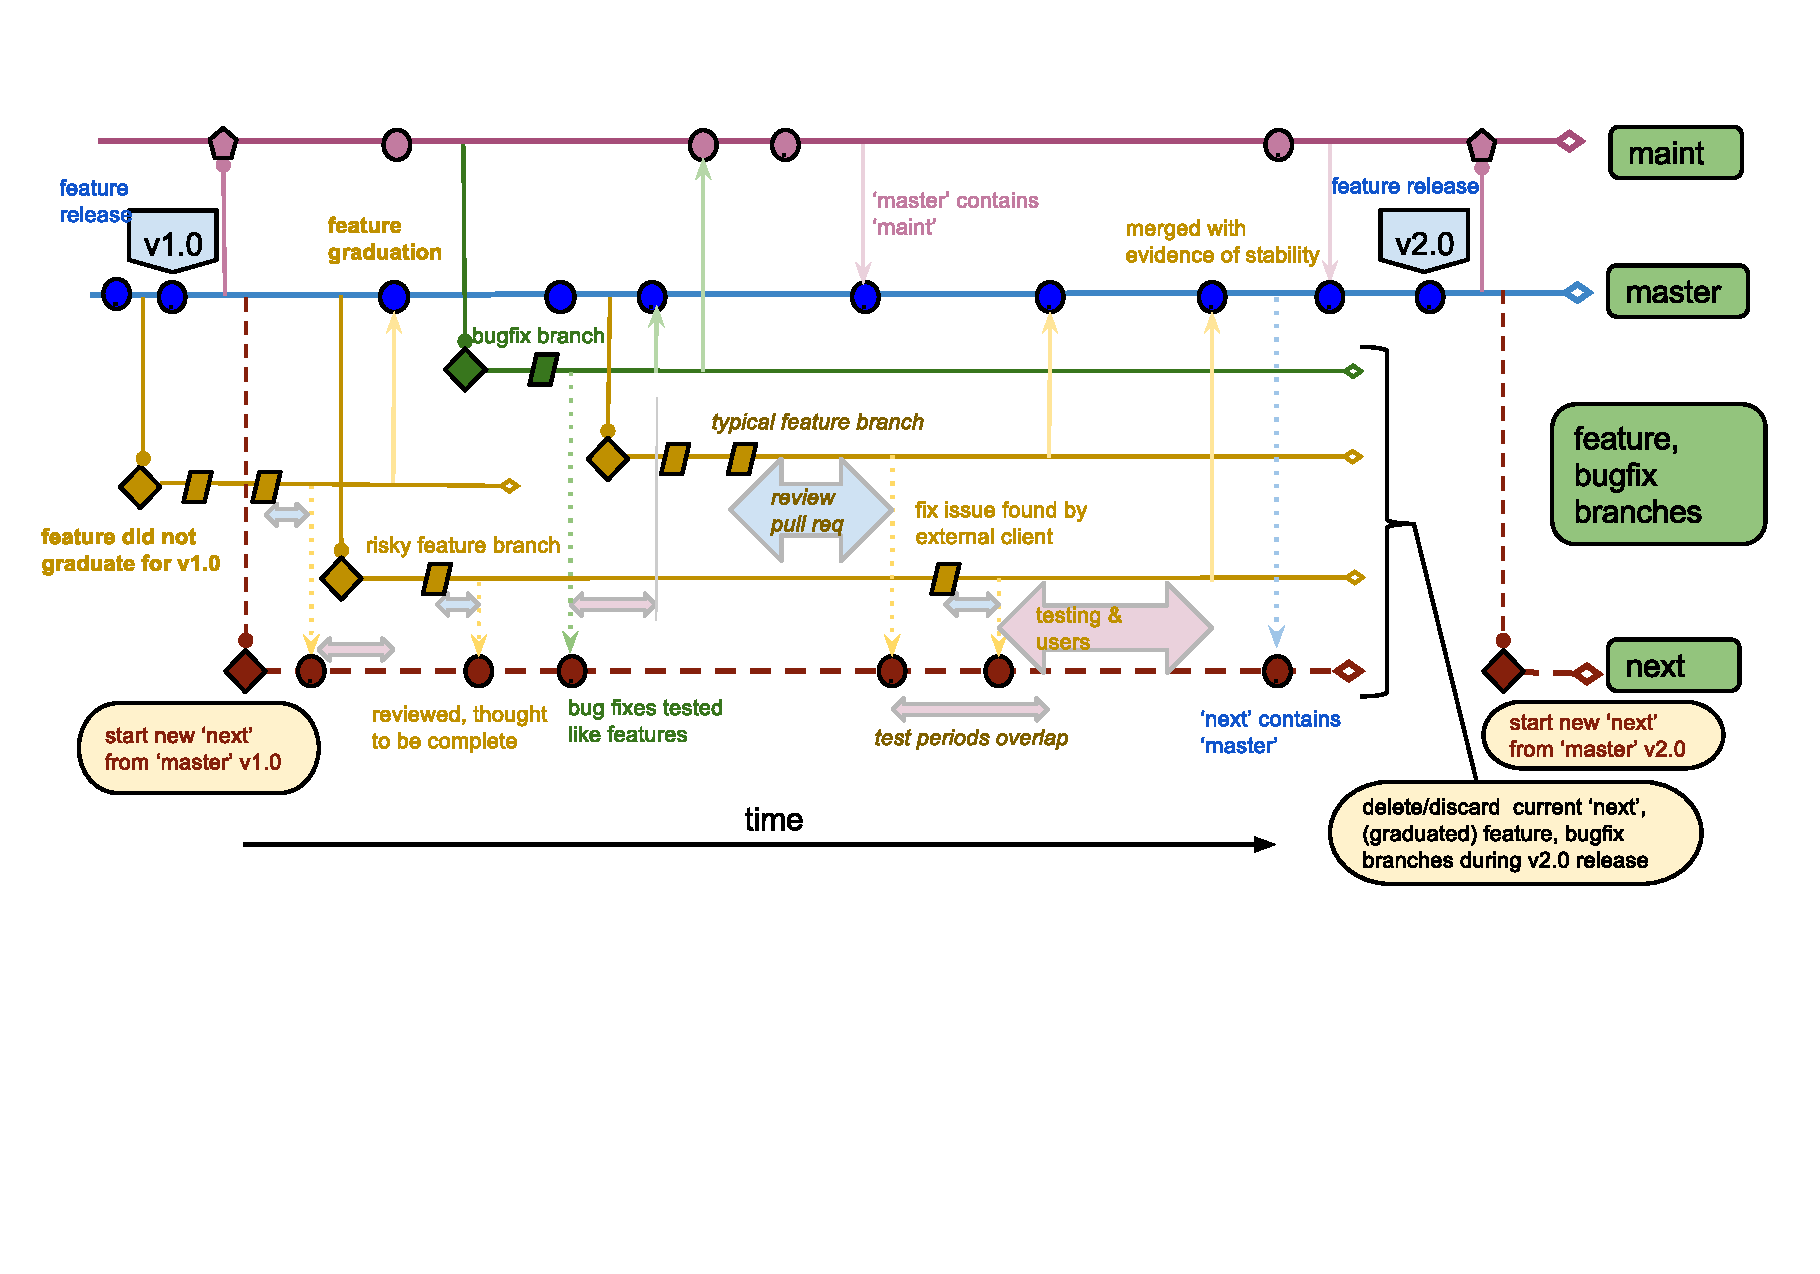
\includegraphics[width=0.99\textwidth]{figures/gitworkflows-95}
  \end{center}
  \begin{flushright} \vspace*{-1.2cm}
   \textit{Git commands are like irregular verbs in a foreign language: \\
           there’s no all-encompassing logic to them, you just have to memorize \\
           which words you need for each thing you want to express}
  \end{flushright}
\end{frame}





%
% Email support
%
\section{PETSc and Emails}

\begin{frame}{PETSc}
   \begin{center} \Large \textbf{What kind of questions do users have?} \end{center}
\end{frame}



\begin{frame}{PETSc and Email Support}
  \begin{block}{Study Setup}
  \begin{itemize}
   \item Classification of Email threads for petsc-user
   \item Years 2006 - 2014
   \item Volume: 904 emails in 2006, 3947 emails in 2014
  \end{itemize}
  \end{block}

  %\pause
  
  \begin{center}
    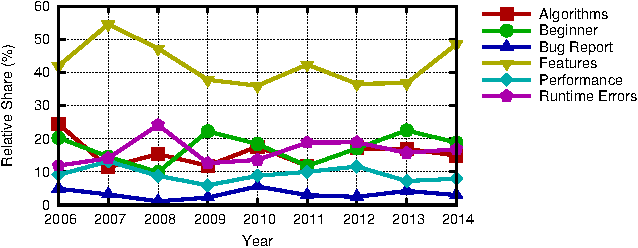
\includegraphics[width=0.85\textwidth]{figures/emails}
  \end{center}

\end{frame}


\begin{frame}{PETSc and Email Support}
  \begin{center}
    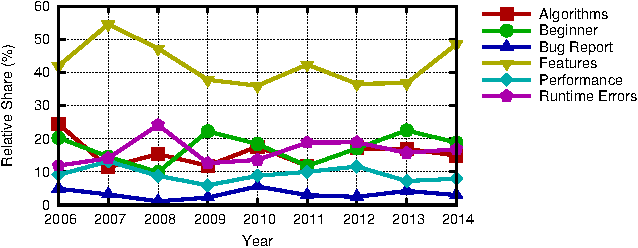
\includegraphics[width=0.85\textwidth]{figures/emails}
  \end{center}

  \begin{block}{Conclusion}
  \begin{itemize}
   \item Involvement of core developers essential
   \item No significant shift in type of support emails
   \item ``Better'' documentation would not change email volume significantly
  \end{itemize}
  \end{block}

\end{frame}






%
% Firetran
%
\section{PETSc and Firetran}

\begin{frame}{PETSc}
   \begin{center} \Large \textbf{What is Firetran?} \end{center}
   %\pause
\vspace*{1cm}
\begin{center}
 
\includegraphics[width=0.9\textwidth]{figures/firetran} \\
 My New Web Browser
\end{center}
\vspace*{1cm}

{ \scriptsize
after J.~Brown, M.~Knepley, B.~Smith: ``Run-time extensibility and librarization of simulation software'' (2015)
}

\end{frame}


%%%%%%%%%%

\begin{frame}[fragile]{Firetran Features}

\begin{block}{Performance}
 \begin{itemize}
  \item 10 percent faster than Firefox ...
  %\pause
  \item ... but no JavaScript
  %\pause
  \item Recompile for JavaScript, performance not shown
  %\pause
  \item Character encoding compiled in for efficiency
 \end{itemize}
\end{block}

\begin{block}{Plugins}
 \begin{itemize}
  %\pause
  \item Directly coded in the core, guarded by \lstinline|#ifdef|
  %\pause
  \item Some ship their own version of Firetran
 \end{itemize}
\end{block}

\begin{block}{Code Quality}
 \begin{itemize}
  %\pause
  \item Some send bug reports
  %\pause
  \item Ignore if not reproducible with my version
 \end{itemize}
\end{block}

\end{frame}


%%%%%%%%%%%

\begin{frame}[fragile]{Firetran Features}

\begin{block}{Convenience}
 \begin{itemize}
  %\pause
  \item Proxy configuration compiled in, don't worry about runtime dialogs
  %\pause
  \item To change: Just edit makefile and recompile
 \end{itemize}
\end{block}


\begin{block}{Security}
 \begin{itemize}
  %\pause
  \item Firetran speaks either http or https
  %\pause
  \item Firetran-http and Firetran-https
 \end{itemize}
\end{block}

\begin{block}{Open Source}
 \begin{itemize}
  %\pause
  \item Development done in private
  %\pause
  \item Release when paper comes out
  %\pause
  \item ``We fixed that in our private repository last year''
  %\pause
  \item Fill out attached form and fax signed copy to view our repository
 \end{itemize}
\end{block}

\end{frame}


%%%%%%%%%%%

\begin{frame}[fragile]{Firetran Features}

\begin{block}{Parental Filter}
 \begin{itemize}
  %\pause
  \item up to 16 pages compiled in
 \end{itemize}
\end{block}


\begin{block}{Building Firetran}
 \begin{itemize}
  %\pause
  \item Build with last year's version of ACME Fortran 77
  %\pause
  \item Build system consists of csh, perl, m4, BSD make
 \end{itemize}
\end{block}

\begin{block}{Navigation}
 \begin{itemize}
  \item No URL bar to save precious screen space
  %\pause
  \item URL entry in configuration file, restart Firetran
  %\pause
  \item Student wrote Tcl script to automate editing and restarting
  %\pause
  \item Script hard to understand, but the way forward
 \end{itemize}
\end{block}

\end{frame}


%%%%%%%%%%%

\begin{frame}[fragile]{Firetran Problems}

\begin{block}{Only One Problem}
 \begin{itemize}
  %\pause
  \item Firetran struggles with market share
 \end{itemize}
\end{block}

%\pause
\begin{block}{Reasons}
 \begin{itemize}
  %\pause
  \item Laughably unacceptable for non-scientific software
 \end{itemize}
\end{block}

\end{frame}

%%%%%%%%%%%


%%%%%%%%%%%

\begin{frame}[fragile]{Firetran Symptoms?}

\begin{block}{Some Linear Algebra and Solver Libraries for Many-Core}
 \begin{itemize}
  \item MAGMA, clMAGMA, MAGMA MIC: CUDA, OpenCL, OpenMP/AVX
  \item MKL: Web tool for linker flags
  \item SuperLU, SuperLU\_dist: Shared vs. distributed memory
  \item Paralution, VexCL: Backend selection at compiletime
  \item ViennaCL: Enable backends at compiletime
  \item (long list to continue...)
 \end{itemize}
\end{block}

%\pause
\begin{block}{Possible Approaches to Fix}
 \begin{itemize}
  \item Raise awareness for usability issues
  \item Incentives for better software engineering
  \item Don't penalize scientists for writing reusable software
 \end{itemize}
\end{block}

\end{frame}




%
% Conclusion and Wrap-Up
%
\section{Conclusions}
\begin{frame}{Conclusions}
 
 \begin{block}{PETSc can Help You}
  \begin{itemize}
   \item Solve algebraic and DAE problems in your application area
   \item Rapidly develop efficient parallel code, can start from examples
   \item Develop new solution methods and data structures
   \item Debug and analyze performance
   \item Advice on software design, solution algorithms, and performance
   \item \centering \texttt{petsc-\{users,dev,maint\}@mcs.anl.gov}

  \end{itemize}
 \end{block}

 \begin{block}{You can Help PETSc}
  \begin{itemize}
   \item Report bugs and inconsistencies, or if you think there is a better way
   \item Tell us if the documentation is inconsistent or unclear
   \item Consider developing new algebraic methods as plugins, contribute if your idea works
  \end{itemize}
 \end{block}

   \begin{flushright}
   \textit{Thank you!}
  \end{flushright}

\end{frame}

